\section{Technique}
\label{sec:technique}

We model configurations as a set of key-value pairs, where
the keys are strings and the values have arbitrary type. This is a
convenient abstraction for analysis as well as a close match for
many standard configuration APIs. It is the abstraction offered
by the POSIX system environment, the Java Properties API,
and the Windows registry.


Figure~\ref{fig:workflow} sketches the high-level workflow of our technique.
Our technique takes as input a program and a list of configuration options.
It first performs a configuration propagation analysis to identify
program elements (here, using the abstraction of predicates) that might be
affected by each configuration (Section~\ref{sec:prop}). Then, it
instruments the original program (Section~\ref{sec:profiling}).

The instrumented version is deployed on the user side to collect program execution
profiles (including both good and bad runs). When the user finds the program
does not work as expected on a given input and configurations,
he/she can invoke the Configuration Deviation Analysis component (Section~\ref{sec:analysis}) to
diagnose the observed behavior. Our technique's output is a ranked list of
configurations that could possibly explain the why the program does not produce the desirable result. Those
configurations, if changed, may even fix the unexpected behavior.

\begin{figure*}[!]
  \centering
  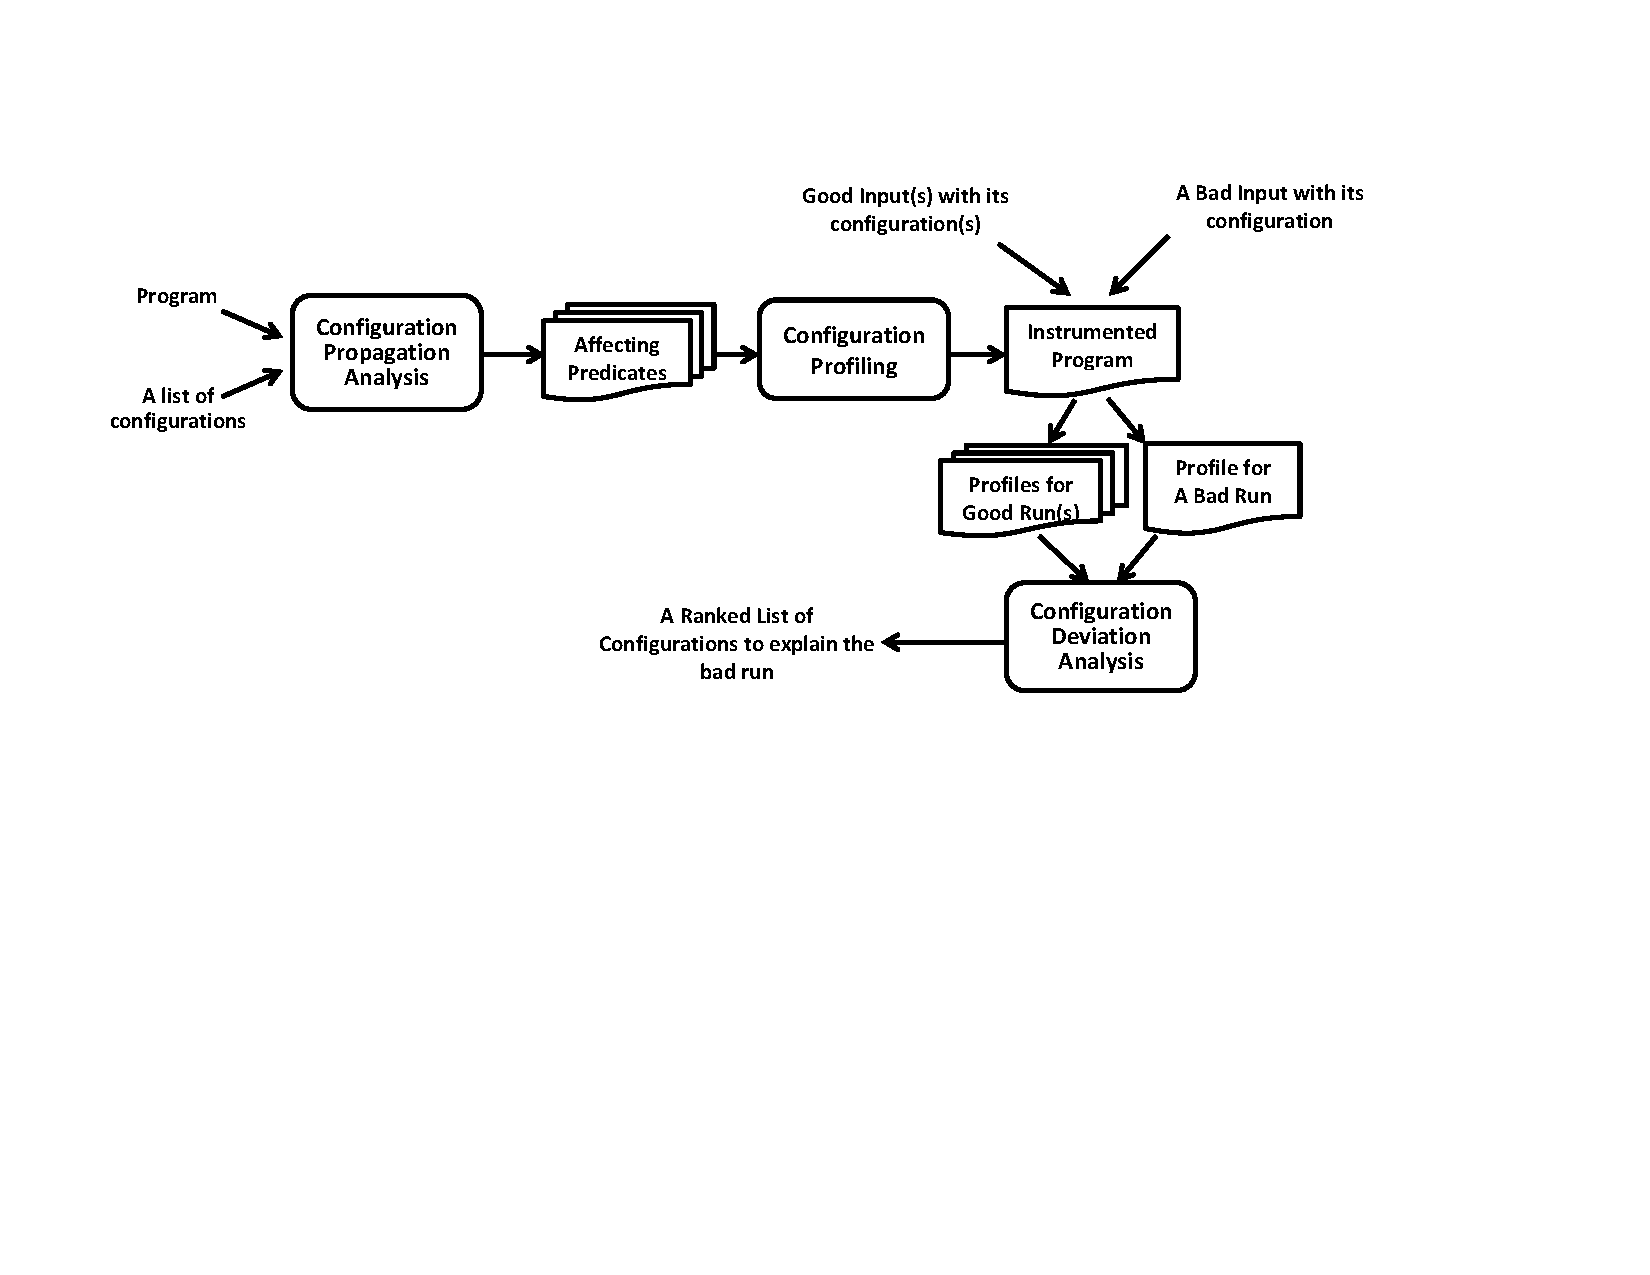
\includegraphics[scale=0.750]{workflow}
  \vspace*{-2.0ex}\caption {{\label{fig:workflow} The workflow of our configuration error explanation technique.
}}
\end{figure*}

\subsection{Configuration Propagation Analysis}
\label{sec:prop}

Given a configuration option, this step statically determines its affected program
elements in the abstraction level of \textit{predicates}. Using predicates
as the abstraction level makes our technique focus on program data flows, instead
of all executed statements.

To identify those affected program predicates, a straightforward way is using program
slicing~\cite{Horwitz:1988:ISU} to compute a forward slice from the assignment statement of the given
configuration option. Unfortunately, traditional slicing includes all statements that
\textit{may} affect a point of interest and often grows too large.

Our technique uses thin slicing~\cite{Sridharan:2007} as a manner to include
\textit{only} statements that are directly affected by the configuration.
We illustrate the advantages of using thin slicing 
 in Figure~\ref{fig:example}.

\begin{figure}[t]
\vspace{-2mm}
\small{//a configuration option to control a sequence's max length}
\vspace{-2mm}
\begin{CodeOut}
\begin{alltt}
int maxsize = readFromCommandLine();  //\textit{seed statement}

1.  public ExecutableSequence step() \ttlcb
2.    ExecutableSequence eSeq = createNewUniqueSequence();
3.    AbstractGenerator.currSeq = eSeq.sequence;
4.    eSeq.execute(executionVisitor);
5.    processSequence(eSeq);
6.    if (eSeq.sequence.hasActiveFlags()) \ttlcb
7.      componentManager.addGeneratedSequence(eSeq.sequence);
8.    \ttrcb
9.    return eSeq;
10. \ttrcb

11. private ExecutableSequence createNewUniqueSequence() \ttlcb
12.   Sequence newSequence = ...; //sequence creation step omitted
13.   if (newSequence.size() > maxsize) \ttlcb
14.     return null;
15.   \ttrcb
16.   if (this.allSequences.contains(newSequence)) \ttlcb
17.     return null;
18.   \ttrcb
19.   return new ExecutableSequence(newSequence);
20. \ttrcb
\end{alltt}
\end{CodeOut}
\tinystep
\vspace*{-3.0ex} \Caption{{\label{fig:example} 
Code excerpt from the Randoop automated test generator~\cite{randoop}.
A forward slice computed by the traditional slicing algorithm~\cite{Horwitz:1988:ISU}
from the seed statement includes statements 2, 3,
4, 5, 6, 7, 9, 13, 14, 16, 17, and 19.
By contrast, a thin slice~\cite{Sridharan:2007}
only contains line 13.
}} %\vspace{-1.8mm}
\end{figure}


\begin{figure}[t]
\begin{CodeOut}
\begin{alltt} 
Configuration option: randoop.main.GenInputsAbstract.maxsize
The predicate: "newSequence.size() > GenInputsAbstract.maxsize" in
"randoop.ForwardGenerator.createNewUniqueSequence()" (line: 312)
shows different behaviors.

In good runs, it evaluates to true:  14.4\% of the time (1315 observations)
In the bad run, it evaluates to true: 32.3\% of the time (2727 observations)

\end{alltt}
\end{CodeOut}
\vspace*{-15pt}
\Caption{{\label{fig:output}
The diagnosis output . The top ranked option 
}} %\vspace{-5mm}
\end{figure}



\textbf{justification of focusing on program control-flow
alternation, rather than values inside.}

The key insight here is that, having no knowledge of
what inputs a user would provide, traditional slicing
captures every single detail of the execution, much
of which is not needed at all by the client.
However, if the provided input changes the workflow,
instead of all data flow into it. 

Take the code exerpt in Figure~\ref{fig:example} as an example.
When Randoop is used to generate tests for different inputs (here,
input mean programs under test), the created tests (method-call
sequence at line 12) would be dramatically different.
However, for similar inputs, the program execution flow should
be similar.

\textbf{justification of focusing on thin slicing, rather
than all affected parts}
Tranditional slicing does not distinguish flows along
pointers from flows along values.

Thin slicing is a technique that focuses on statements
that flow values to the seed, ignoring the uses of
base pointers.

A thin data dependence graph has exactly
the same set of nodes as its corresponding data dependence
graph. However, for an access \CodeIn{v.f}, the base pointer value
in \CodeIn{v} is not considered to be used. 

This property makes thin slicing
especially attractive.

Also Take the code in Figure~\ref{fig:example} as an example.
Use traditional slicing to compute all affected statement,
the configuration option \CodeIn{maxsize} would affect
branching statement 6, 13, and 16. However, the
statements 6 and 13 are incorrectly identified, since
whether a sequence has an active flag (line 6) or
whether a sequence has been executed before (line 16)
has nothing to do with the \CodeIn{maxsize} configuration option.
In fact, there is another configuration option $\blacksquare$
that affect line 6.

% improves the relevance
%of the slice by focusing on the statements that compute
%and copy a value to the seed.

By separating pointer computations from value flow,
this approach naturally connects configurations and its
directly affected statements.


\subsection{Configuration Behavior Profiling}
\label{sec:profiling}

For each configuration, after obtaining its affected predicates, our technique
instruments the program \textit{only} on those affected predicates. The instrumentation
code keeps the results of how an affected predicate evaluates at runtime. Besides keeping
the predicate evaluation results, the instrumentation code also keeps
the calling context information.

Take the code excerpt in Figure~\ref{fig:example} as an example, the affected
predicate of configuration option \CodeIn{maxszie} is at line 13. Thus, our technique
only instruments line 13, producing the instrumented
code as follows (the instrumentation code is highlighted by underline):


\begin{CodeOut}
\begin{alltt}
11. private ExecutableSequence createNewUniqueSequence() \ttlcb
12.   Sequence newSequence = ...; //sequence creation step omitted
      \underline{Instrumenter.beforeEvaluation(maxSize);}
      \underline{Instrumenter.saveCallingContext(maxSize);}
13.   if (newSequence.size() > maxsize) \ttlcb
        \underline{Instrumenter.evaluateToTrue(maxSize);}
14.     return null;
      ...
20. \ttrcb
\end{alltt}
\end{CodeOut}

The helper class \CodeIn{Instrumenter} saves the calling context (i.e.,
method-call chains from the main entry), and the predicate evaluation result.

Take the Randoop code in Figure~\ref{fig:example} as an example. Suppose when
generating tests for a given program, 100 sequences are created (line 12) and 20
of them exceed the max length as specified in the \CodeIn{maxSize} configuration option.
As a result, the predicate at line 13 is evaluated 100 times, among which 20 times the
predicate evaluates to \CodeIn{true}. Therefore,
our instrumentation code will record the following information as profile for the predicate
at line 13:

%\pagebreak

\begin{CodeOut}
\begin{alltt}
configuration: maxsize
context: main -> ... -> step() - > createNewUniqueSequence()
predicate: newSequence.size() > maxsize
    \# evaluation: 100
    \# true branch: 20
    \# false branch: 80
\end{alltt}
\end{CodeOut}

\subsection{Configuration Deviation Analysis}
\label{sec:analysis}


Introduce the metric for ranking configurations, and its
statistical meaning,e g., balance 2 parts

\subsubsection{Non-Crashing Problems}

\subsubsection{Crashing Problems}

When some unexpected program behavior is observed, our technique
attempts to explain its reason by comparing the recorded profile (denoted
as \textit{bad-run profile}) with the recorded profiles of all
executions on similar inputs that produced expected results (denoted as \textit{good-run profiles}).

The configuration deviation analysis selects configuration
options whose bad-run profile deviate most from its good-run profiles.

Suppose, a bad run produces the following profile (2 configurations: \CodeIn{maxsize}
and \CodeIn{repeat\_heuristic}. Calling context is omitted for brevity.):

\begin{CodeOut}
\begin{alltt}
configuration: maxsize 
predicate: newSequence.size() > maxsize
    \# evaluation: 100
    \# true branch: 60
    \# false branch: 40

configuration: repeat_heuristic
predicate: repeat_heuristic
    \# evaluation: 50
    \# true branch: 50
    \# false branch: 0
\end{alltt}
\end{CodeOut}

For a good run with a similar input, the following profile is observed:

\begin{CodeOut}
\begin{alltt}
configuration: maxsize 
predicate: newSequence.size() > maxsize
    \# evaluation: 100
    \# true branch: 20
    \# false branch: 80

configuration: repeat_heuristic
predicate: repeat_heuristic
    \# evaluation: 50
    \# true branch: 50
    \# false branch: 0
\end{alltt}
\end{CodeOut}

Our technique determines that in a good run, the ratio of predicate 
\CodeIn{newSequence.size() > maxsize} being evaluated to true is: 20 / 80 = 0.2;
but in a bad run, the ratio of the same predicate being evaluated to true is: 60 / 100 = 0.6.
On the other hand, the ratio of the other predicate (i.e., \CodeIn{repeat\_heuristic}) being evaluated to true
remains the same in both good and bad runs. Therefore, the behavior
of predicate \CodeIn{newSequence.size() > maxsize} deviates most, and our technique
selects the \CodeIn{maxsize} configuration as the responsible one, and displays it to the user, suggesting he/she
to inspect its value and re-set it.

\subsection{Discussion}
Why dynamic slicing is not usable? No seed statement, and great overhead. Using JSlicer incurs
a great overhead. It needs to track every instruction and
perform synchronization when dependence graph is updated.

Our technique can be seen as a way to reduce overhead,
including selective profiling, and static pre-processing
techniques.

